%----------------------------------------------------------------------------------------
%	PACKAGES AND OTHER DOCUMENT CONFIGURATIONS
%----------------------------------------------------------------------------------------
\documentclass[11pt]{article}

\usepackage{lastpage} % Required to determine the last page for the footer
\usepackage{extramarks} % Required for headers and footers
\usepackage{graphicx} % Required to insert images
\usepackage{lipsum} % Used for inserting dummy 'Lorem ipsum' text into the template
\usepackage{hyperref}
\usepackage{float}
\usepackage[bottom]{footmisc}
\usepackage{subcaption}
\usepackage{listings}
\usepackage{amsmath}
\usepackage{color}
\usepackage[ruled,vlined]{algorithm2e}
\usepackage{pdflscape}

\linespread{1.1} % Line spacing
\usepackage[total={6in, 8in}]{geometry}

\setlength\parindent{0pt} % Removes all indentation from paragraphs

%set c++ settings for adding in code snippets
\lstset{language=C++,
                basicstyle=\ttfamily,
                keywordstyle=\color{blue}\ttfamily,
                stringstyle=\color{red}\ttfamily,
                commentstyle=\color{cyan}\ttfamily
}

\begin{document}

\subsection{Process Evaluation}
In this section I take time to evaluate my implementation process, aside
from the results gathered from the final product.

\subsubsection{OpenCV}
Using third party libraries is always a gamble, their performance is not
always guaranteed. Even for a library so well supported as OpenCV, there 
were times where the library did not behave as expected. This can be 
attributed to some of the algorithms used in the functions provided. 
Whether there exists a more suitable and better performing algorithm is
unlikely and hard to determine.\\
\\
Having justified my use of the OpenCV library, playing around with a 
few functions and digging through the documentation to see what was
on offer for me, I think it was the best option to use. 
However, I did not conduct a thorough enough investigation into specific
functions and their behaviour. This would have merited a lot more time in 
the beginning of the project, it would not have changed my mind to  use
the library but would have prepared me against some of the problems that 
arose throughout the project. The Computer Vision aspect is the most
important part in my project, it is the first step and an inaccurate
representation of the drawn scene will cause the rest of the 
implementation and the result to be inaccurate and essentially useless. As
a result, OpenCV played a huge part in this project. 
In this section, I outline some of the
problems that came with using OpenCV, a brief explanation of my solution
(of which more can be read about in Section \ref{lol}), and evaluation of
the solution. 

\subsubsection{Contour Detection}
The first major step in this project is contour detection. This was achieved
using the Canny Detector from OpenCV, thresholding empirically. Having
researched edge detectors avaiilable to me before hand, I was aware of those
available and I could manipulate the output in various ways by
changing the paramters passedto the function. I did experiment with different
sizes of Sobel kernel, which were 3x3, 5x5 and 7x7. In addition, I also
tested various upper and lower thresholds which are used for hysteresis. The
results were accumulated as pictures and I stored the output for visual
comparison. After this process was done I made my choice of threshold values
and kernel size based on which pictures seemed to capture the contours
in each contour the best. \\
\\
Figure \ref{fig:kernelDetermining} shows the way I determined the best kernel
size. I simultaneously raised the Upper and lower thresholds alongside the 
kernel size so that I could visually compare them later on. I did this
across different pictures as well, with different styles of contours drawn,
thick, thin, open etc. The Sobel operator has a smoothing effect when
used and so its size will affect contour detection quality.
From this I found that the best kernel size to use was
a 5x5 kernel. The best picture to illustrate this is \ref{kernelExample1} 
and \ref{kernelExample2}, Looking at the smaller, circular contour in
\ref{kernelExample1}, it is coloured red, with its inner contour
blue and then the inner contour's inner area coloured red. This highlights
3 distinct contours identified. In \ref{kernelExample2} the same contour
now only has two colours, the outer most being blue with the inner, inner
area being red. This is because the inner contour has been joined with the
outer contour as the kernel size was too large and determined the two
contours to be connected! In the other case, in \ref{kernelExample3}, the
same contour did not have its inner, inner area coloured, this  because the
kernel size was too small and did not join the contour completely. In 
addition, the simple square in \ref{kernelExample3}, just to the top right of
the large, curved contour, has its edges coloured green
and red, whilst both \ref{kernelExample2} and \ref{kernelExample3} correctly
detect the square to be one contour, coloured in a single colour. Since
the program should be able to tolerate some small amount of openness of
contours, the kernel size was determined, empirically, best of size 5.

\begin{figure}[!h]
\centering
	\begin{subfigure}[t]{.25\textwidth}
		\centering
		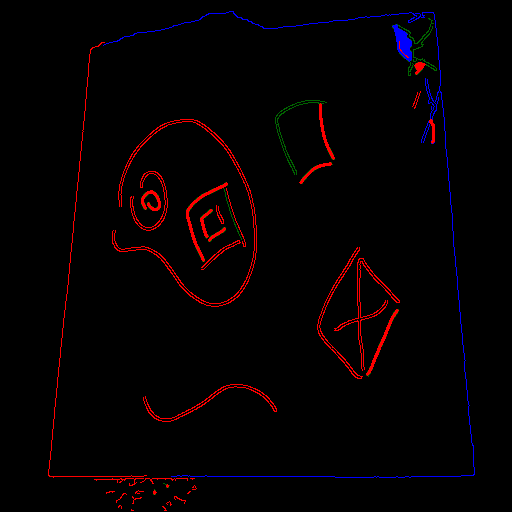
\includegraphics[scale=0.3]
		{pics/shitlinesThreshTest/Upper1700lower1000kernel3.png}
		\caption{U:1700, L:1000, K:3x3}
	\end{subfigure}
\hfill
	\begin{subfigure}[t]{.25\textwidth}
		\centering
		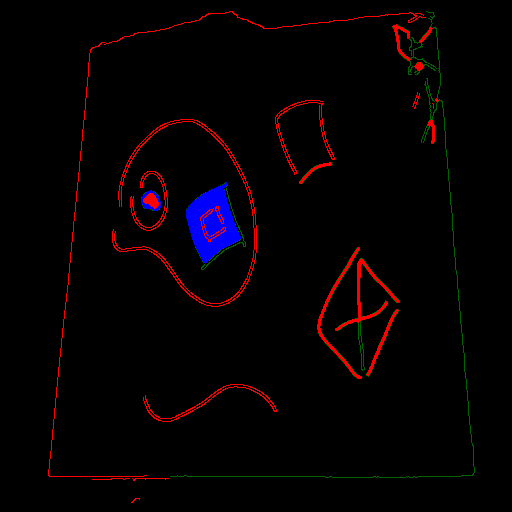
\includegraphics[scale=0.3]
		{pics/shitlinesThreshTest/Upper1700lower1000kernel5.png}
		\caption{U:1700, L:1000, K:5x5}
	\end{subfigure}
\hfill
	\begin{subfigure}[t]{.25\textwidth}
		\centering
		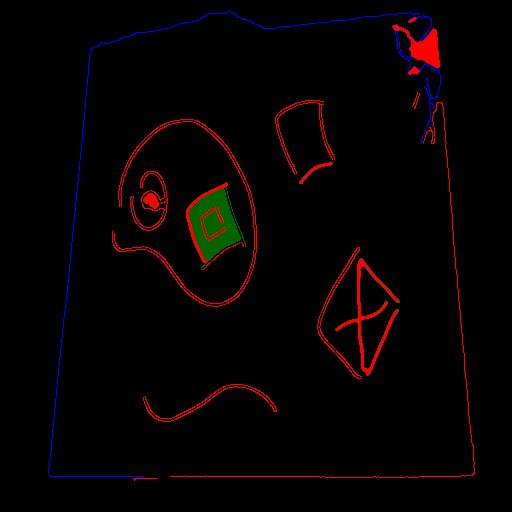
\includegraphics[scale=0.3]
		{pics/shitlinesThreshTest/Upper1700lower1000kernel7.png}
		\caption{U:1700, L:1000, K:7x7}	
	\end{subfigure}


	\begin{subfigure}[t]{.25\textwidth}
		\centering
		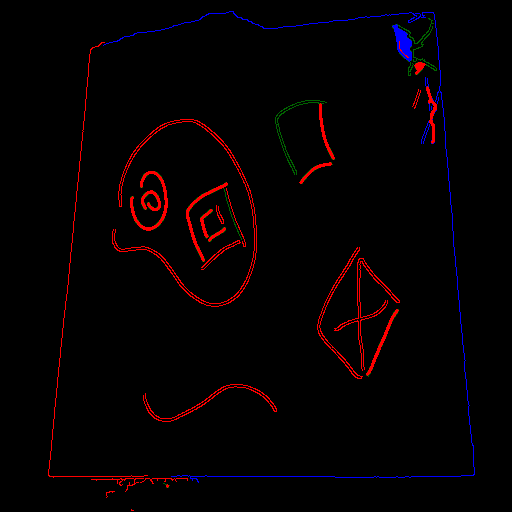
\includegraphics[scale=0.3]
		{pics/shitlinesThreshTest/Upper2200lower800kernel3.png}
		\caption{U:2200, L:800, K:3x3}
		\label{kernelExample3}
	\end{subfigure}
\hfill
	\begin{subfigure}[t]{.25\textwidth}
		\centering
		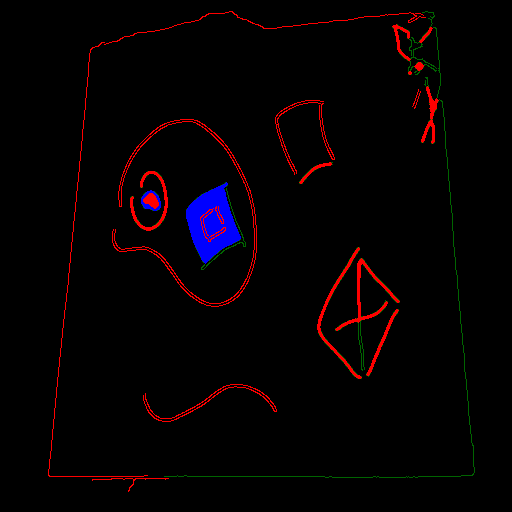
\includegraphics[scale=0.3]
		{pics/shitlinesThreshTest/Upper2200lower800kernel5.png}
		\caption{U:2200, L:800, K:5x5}
		\label{kernelExample1}
	\end{subfigure}
\hfill
	\begin{subfigure}[t]{.25\textwidth}
		\centering
		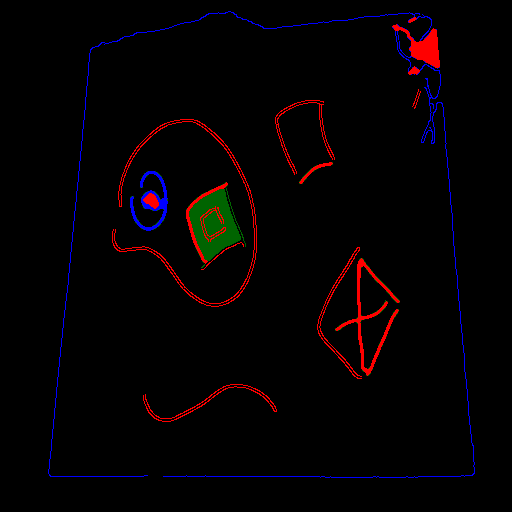
\includegraphics[scale=0.3]
		{pics/shitlinesThreshTest/Upper2200lower800kernel7.png}
		\caption{U:2200, L:800, K:7x7}
		\label{kernelExample2}
	\end{subfigure}


	\begin{subfigure}[t]{.25\textwidth}
		\centering
		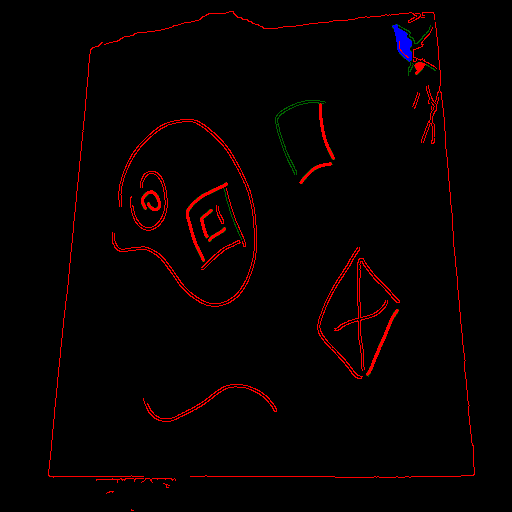
\includegraphics[scale=0.3]
		{pics/shitlinesThreshTest/Upper2200lower1200kernel3.png}
		\caption{U:2200, L:1200, K:3x3}
	\end{subfigure}
\hfill
	\begin{subfigure}[t]{.25\textwidth}
		\centering
		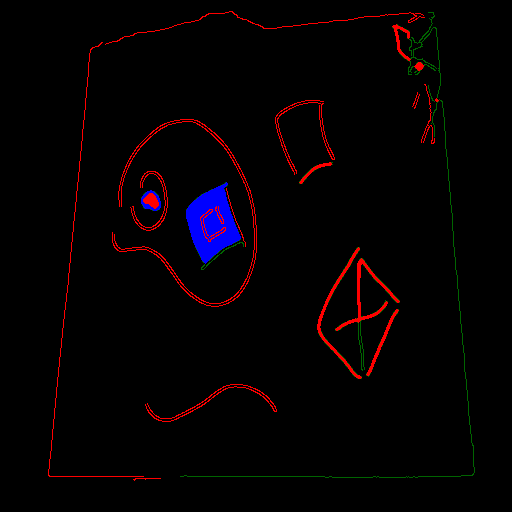
\includegraphics[scale=0.3]
		{pics/shitlinesThreshTest/Upper2200lower1200kernel5.png}
		\caption{U:2200, L:1200, K:5x5}
	\end{subfigure}
\hfill
	\begin{subfigure}[t]{.25\textwidth}
		\centering
		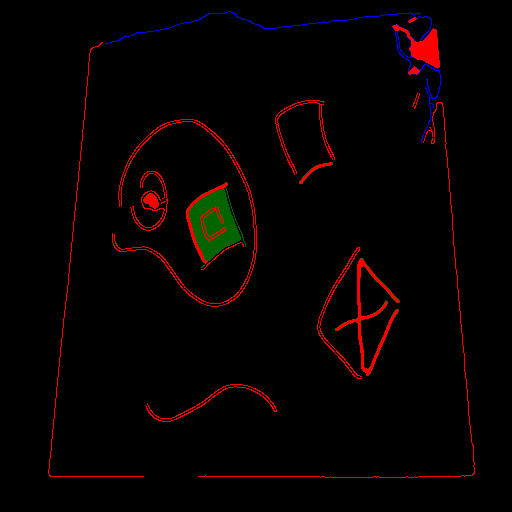
\includegraphics[scale=0.3]
		{pics/shitlinesThreshTest/Upper2200lower1200kernel7.png}
		\caption{U:2200, L:1200, K:7x7}
	\end{subfigure}
	
	\caption{Example of determining Kernel size \\
		(U = UpperThreshold, L = LowerThreshold, K = KernelSize)}
	\label{fig:kernelDetermining}
\end{figure}


Figure \ref{fig:hysteresisDetermining} shows a
small selection of results I obtained through this kind of testing. After
seeing that performance was best between an upper threshold of 1700 and 2200,
along with a lower threshold of 800, I did a smaller scale, binary search
approach to reach the upper and lower thresholds the program currently uses
of 2000 and 900 respectively

\begin{figure}[!h]
\centering
	\begin{subfigure}[t]{.25\textwidth}
		\centering
		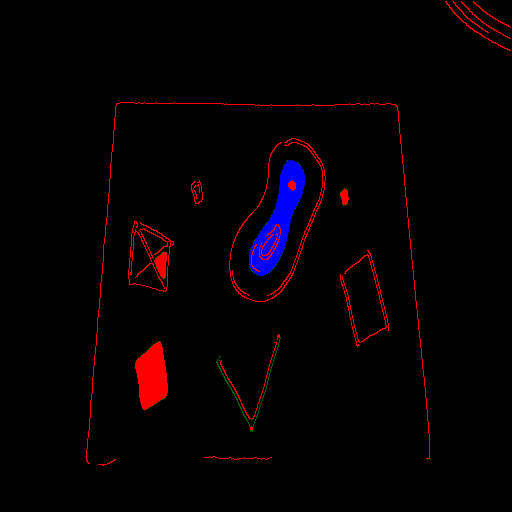
\includegraphics[scale=0.3]{pics/normalThreshTest/Upper1700lower800kernel5.png}
		\caption{U:1700, L:800}
	\end{subfigure}
\hfill
	\begin{subfigure}[t]{.25\textwidth}
		\centering
		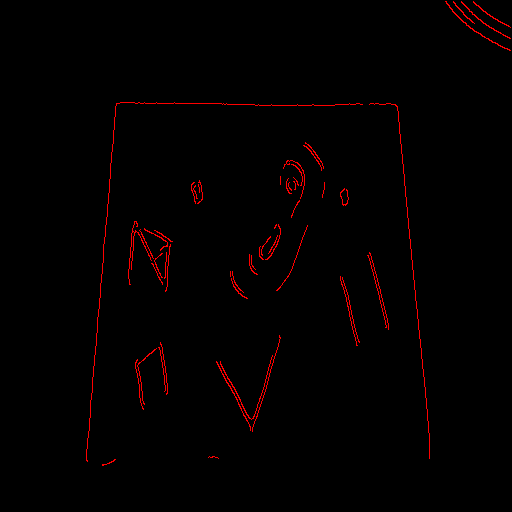
\includegraphics[scale=0.3]{pics/normalThreshTest/Upper1700lower1200kernel5.png}
		\caption{U:1700, L:1200}
	\end{subfigure}
\hfill
	\begin{subfigure}[t]{.25\textwidth}
		\centering
		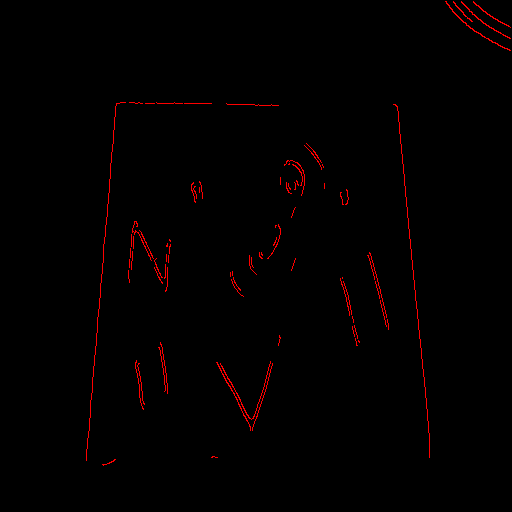
\includegraphics[scale=0.3]{pics/normalThreshTest/Upper1700lower1400kernel5.png}
		\caption{U:1700, L:1400}	
	\end{subfigure}


	\begin{subfigure}[t]{.25\textwidth}
		\centering
		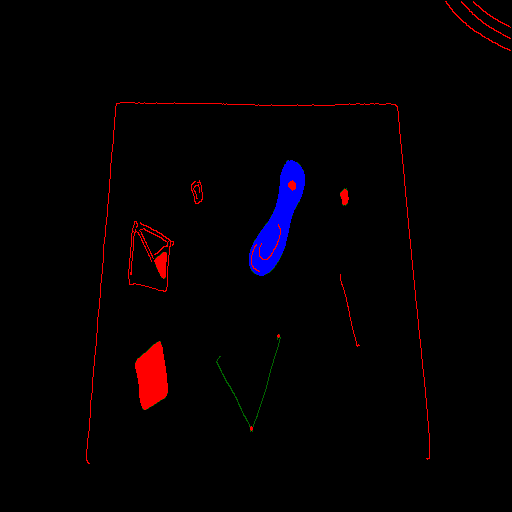
\includegraphics[scale=0.3]{pics/normalThreshTest/Upper2200lower800kernel5.png}
		\caption{U:2200, L:800}
	\end{subfigure}
\hfill
	\begin{subfigure}[t]{.25\textwidth}
		\centering
		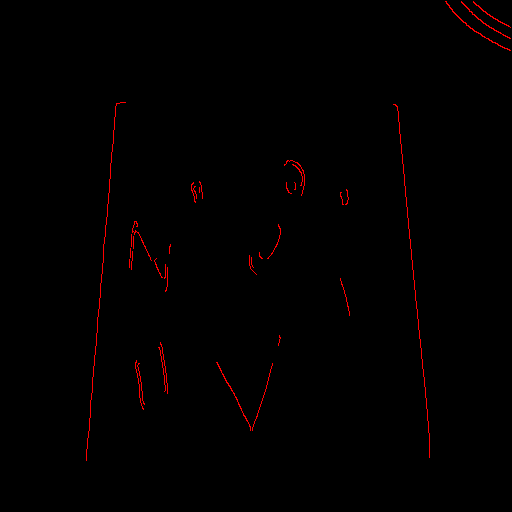
\includegraphics[scale=0.3]{pics/normalThreshTest/Upper2200lower1400kernel5.png}
		\caption{U:2200, L:1400}
	\end{subfigure}
\hfill
	\begin{subfigure}[t]{.25\textwidth}
		\centering
		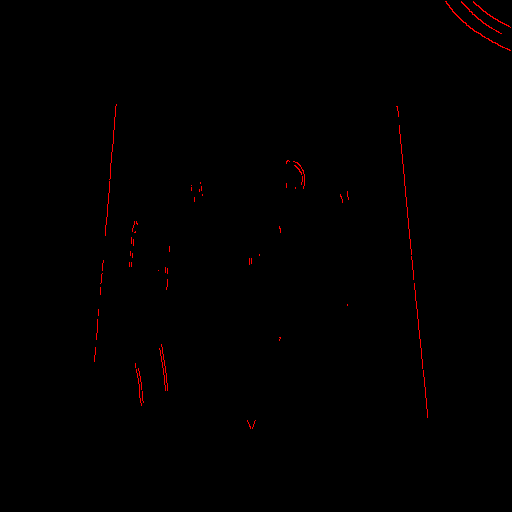
\includegraphics[scale=0.3]{pics/normalThreshTest/Upper2200lower2000kernel5.png}
		\caption{U:2200, L:2000}
	\end{subfigure}

	
	\begin{subfigure}[t]{.25\textwidth}
		\centering
		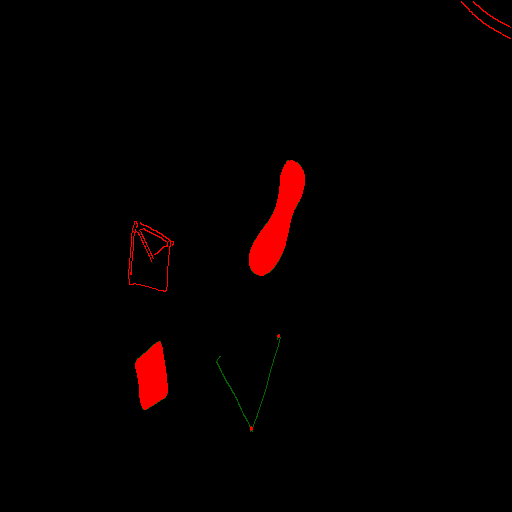
\includegraphics[scale=0.3]{pics/normalThreshTest/Upper2700lower800kernel5.png}
		\caption{U:2700, L:800}
	\end{subfigure}
\hfill
	\begin{subfigure}[t]{.25\textwidth}
		\centering
		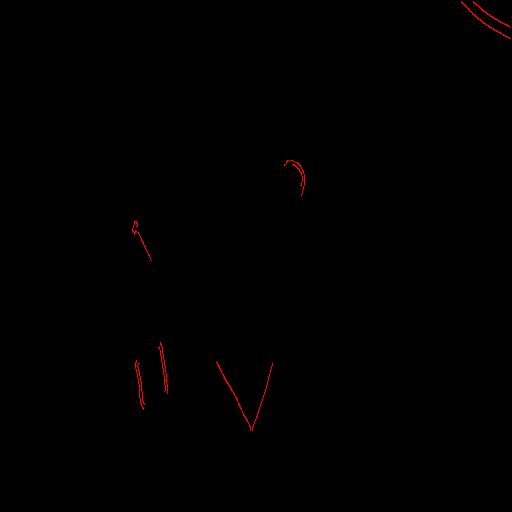
\includegraphics[scale=0.3]{pics/normalThreshTest/Upper2700lower1400kernel5.png}
		\caption{U:2700, L:1400}
	\end{subfigure}
\hfill
	\begin{subfigure}[t]{.25\textwidth}
		\centering
		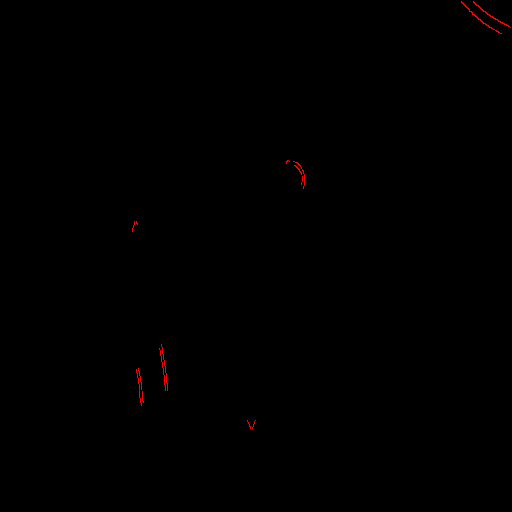
\includegraphics[scale=0.3]{pics/normalThreshTest/Upper2700lower2000kernel5.png}
		\caption{U:2700, L:2000}
	\end{subfigure}
	
	\caption{Example of determining hysteresis thresholds with kernel size = 5. \\(U = UpperThreshold, L = LowerThreshold}
	\label{fig:hysteresisDetermining}
\end{figure}

A regret I have with the way I tackled detecting contours is not fully 
investigating using pure thresholding to identify contours. Quite naively, 
after reading
up the Canny edge detector versus other edge detection algorithms, I tunnel
visioned on that solution because I thought it was the best of the edge 
detectors. However, I did not consider the thought of not using
a edge detecor, just simply using a thresholding algorithm that if pixels 
vary in intensity from those nearby, mark it as a possible contour. I
missed the fact that I could purely use thresholding to identify possible
contours and use the result to form a hierarchy. However, in retrospect,
whether this approach would have worked better than using the Canny 
remains to be determined. It may
have behaved a lot worse, I would also have to spend a lot of time 
empirically determining the threshold values, especially without the 
use of hysteresis which is so useful in the Canny Edge Detector. However, if
the user was limited to using just black pen on a white paper surface,
detection of contours may have done well in the thresholding case. However,
with these points in mind, I think it was sufficient to try out the 
Canny detection method, due to its proven good performance by using
the double thresholding method with hysteresis. Detecting contours
without an edge detector could be a worthwhile extension or something that
future projects should consider in their approaches.

\subsubsection{Contour Joining}
OpenCV offers a method, \texttt{findContours()} which will return a
vector of contours (expressed as a vector of constituent points) along with
a hierarchy describing the relation of these contours. However, detection
isn't always perfect sometimes a contour, though continuous on paper
will be identified as several contours. In an attempt to reduce this, I 
use morphological closing to try connect contours as much as possible.
This worked to some extent but had to be amplified with another join
algorithm. The algorithm I implemented was to analyse the beginning and end points
of each contour, due to the order in which OpenCV discovers, it is sufficient 
enough to join contours that are subsequent to others in the returned
vector. If two adjacent contours are within an empirically set pixel
neighbourhood they will be joined together. \\
\\
When using the \texttt{findContours()} if a contour is not closed,
points, in an effort to close the contour, the library will duplicate 
points as a way to get from the end of the contour back to the beginning
point without loss of information. However, sometimes the backtrack does
deviate from the original beginning-to-end point path and choose a very
slightly different path on the way back to the beginning point. This causes 
a variety of complications, if we were to naively remove duplicate points
within each contour, there may be stray points on the contour that do not
belong. This is best explained in the example below in Figure \ref{backtrack}.
The coloured pixels indicate a possible contour. Consider this contour
starting left and ending right, this is not a closed contour and
so OpenCV tries to close it. The mauve pixels are pixels that are part
of the front and back traversal. On the way back the constituent pixels
deviate slightly due to detection in OpenCV. The black pixels are
on the path left to right, the pink pixels are those on the path right to left.
By eliminating duplicates, we will keep the pink pixels. If these are on the
way back and pixel discovery order is preserved, then the pink pixels are
where the contour will "end" as determined by OpenCV rather than at the 
original start point. This causes a massive problem later on where we
will be unable to tell if contours are actually closed or not and connecting
nearby contours becomes a problem since they no longer have their
start and end points nearby each other. After assessing the behaviour of 
the program after trying to eliminate duplicate points in conjunction 
with my \texttt{naivecontourjoin()} algorithm, I found these exact
problems to occur, making joining contours almost impossible. As it
would be better to reduce the amount of contours by joining them, my approach
to this problem was to simply leave the duplicated points as they would 
at least preserve the original contour end and begin properties. This is
something that should be considered by others thinking of working with
OpenCV for contour detection.

\begin{figure}[!h]
	\centering
	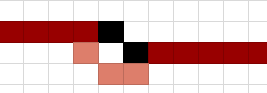
\includegraphics[scale=0.8]{pics/backtrack.png}
	\caption{Contour Backtracking problem}
	\label{backtrack}
\end{figure}

\subsubsection{TODO ~ Contour Elimination}
For the landscape seen in Figure \ref{eliminationInput}, the results of
runnig \texttt{findContours()} can be seen in 
Figure \ref{fig:contourElimination}. In Figure \ref{eliminationInput}, we
clearly see that there are only 3 contours, OpenCV finds 21 contours. These
can be attributed to the fact that contours are counted twice (once entering
the contour, once leaving the contour) in addition to the ArUco marker being
treated as a contour. In addition, there are other contours found that are
a lot more subtle, some of these are joined with the \texttt{naivecontourjoin()}
algorithm as explained in the last section. Joining the contours
reduces the total count to 13 so my approach above does work quite well, but
there are still anomalies that will take more than just proximity checking
to join together. 

\begin{figure}[!h]
	\centering
	\begin{subfigure}[t]{0.45\textwidth}
		\centering
		
\includegraphics[scale=1.4]{pics/elimination.jpg}
		\caption{Landscape Map}
		\label{eliminationInput}
	\end{subfigure}
	\hfill
	\begin{subfigure}[t]{0.45\textwidth}
		\centering
		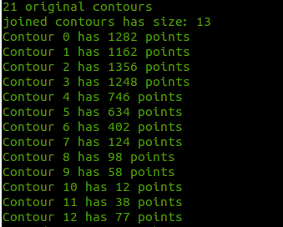
\includegraphics[scale=0.8]{pics/eliminationResults.png}
		\caption{Contours Found}
		\label{eliminationResults}
	\end{subfigure}
	\caption{Results of \texttt{findContours()}}
	\label{elimination}
\end{figure}

There were other algorithms implemented within this project to try to reduce the
contour count. This is because having a smaller contour tree will speed
up the overall computation in the program. The first of which was to try and
eliminate contours of negligible size. Looking at Figure \ref{eliminationResults},
we ca see cotour 9,10 and 11 have considerably less contours than the
other ones found, having under 60 points each. The original intuition is that
these can be thrown away with minimal impact on the understanding of the
landscape map. This is further backed up by the fact that they add
minimal extra value to the reconstruction of the landscape map in contour form,
which is seen in Figure \ref{construction}.\\
\\
As can be seen from Figure\ref{construction9}, Figure \ref{construction10} and
Figure \ref{construction11}. There is not much gained from keeping the smaller
contours. In addition, Figure \ref{construction12} also seems negligible, with
the final construction seemingly done by Figure \ref{construction8}. 

\begin{figure}
	\centering
	\begin{subfigure}[t]{0.32\textwidth}
	\centering
		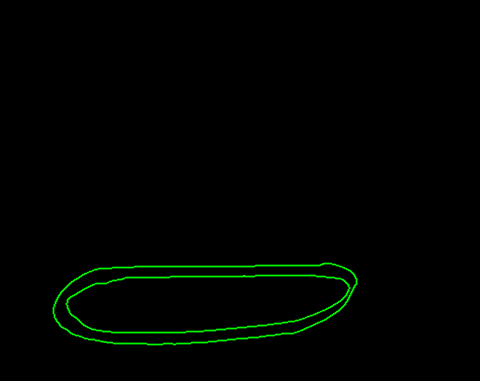
\includegraphics[scale=0.28]{pics/elimination/joinedAfterRemoval1.png}
		\caption{1}
		\label{construction1}
	\end{subfigure}
	\begin{subfigure}[t]{0.32\textwidth}
	\centering
		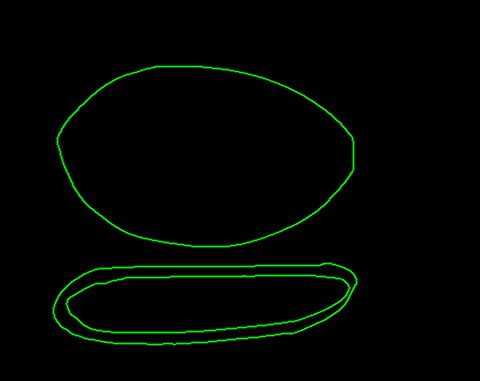
\includegraphics[scale=0.28]{pics/elimination/joinedAfterRemoval2.png}
		\caption{1,2}
		\label{construction2}
	\end{subfigure}
	\begin{subfigure}[t]{0.32\textwidth}
	\centering
		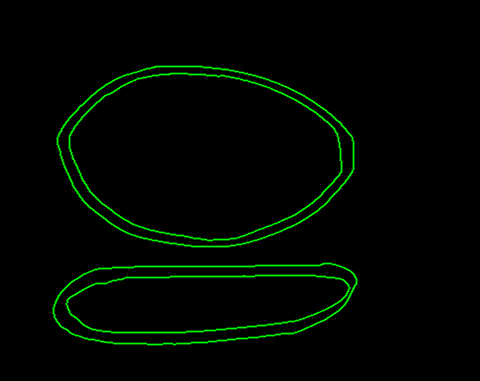
\includegraphics[scale=0.28]{pics/elimination/joinedAfterRemoval3.png}
		\caption{1,2,3}
		\label{construction3}
	\end{subfigure}
	
	
	\begin{subfigure}[t]{0.32\textwidth}
	\centering
		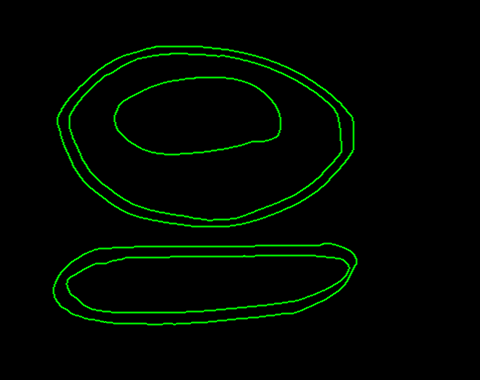
\includegraphics[scale=0.28]{pics/elimination/joinedAfterRemoval4.png}
		\caption{1,2,3,4}
		\label{construction4}
	\end{subfigure}
	\begin{subfigure}[t]{0.32\textwidth}
	\centering
		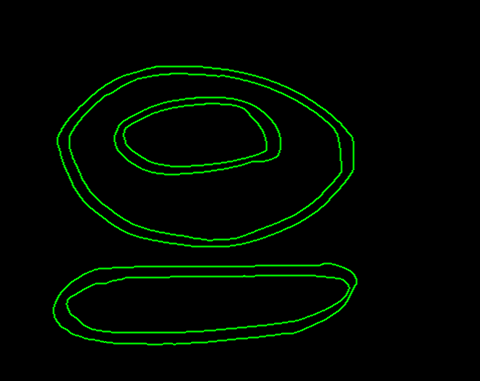
\includegraphics[scale=0.28]{pics/elimination/joinedAfterRemoval5.png}
		\caption{1 to 5}
		\label{construction5}
	\end{subfigure}
	\begin{subfigure}[t]{0.32\textwidth}
	\centering
		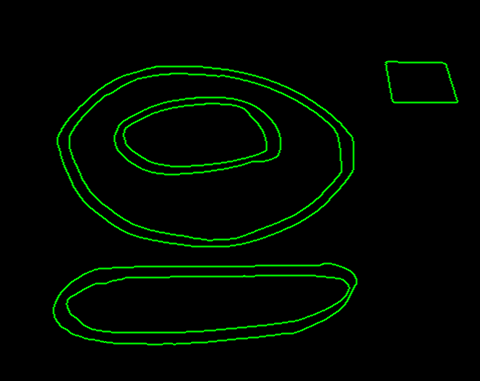
\includegraphics[scale=0.28]{pics/elimination/joinedAfterRemoval6.png}
		\caption{1 to 6}
		\label{construction6}
	\end{subfigure}

	
	\begin{subfigure}[t]{0.32\textwidth}
	\centering
		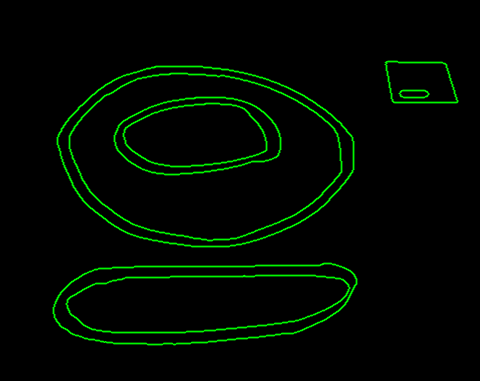
\includegraphics[scale=0.28]{pics/elimination/joinedAfterRemoval7.png}
		\caption{1 to 7}
		\label{construction7}
	\end{subfigure}
	\begin{subfigure}[t]{0.32\textwidth}
	\centering
		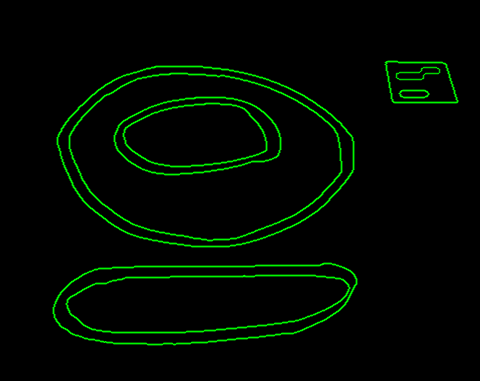
\includegraphics[scale=0.28]{pics/elimination/joinedAfterRemoval8.png}
		\caption{1 to 8}
		\label{construction8}
	\end{subfigure}
	\begin{subfigure}[t]{0.32\textwidth}
	\centering
		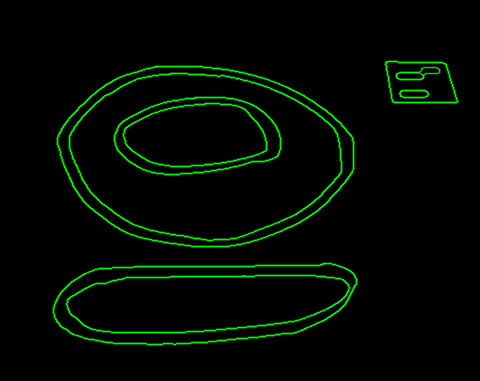
\includegraphics[scale=0.28]{pics/elimination/joinedAfterRemoval9.png}
		\caption{1 to 9}
		\label{construction9}
	\end{subfigure}

	
	\begin{subfigure}[t]{0.32\textwidth}
	\centering
		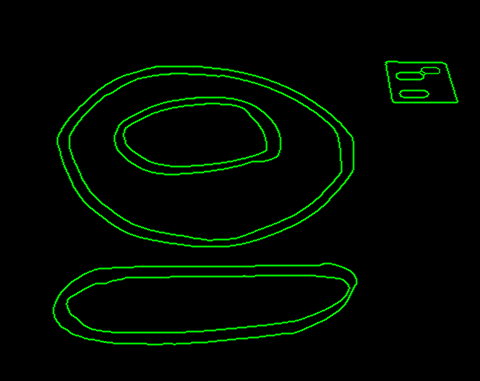
\includegraphics[scale=0.28]{pics/elimination/joinedAfterRemoval10.png}
		\caption{1 to 10}
		\label{construction10}
	\end{subfigure}
	\begin{subfigure}[t]{0.32\textwidth}
	\centering
		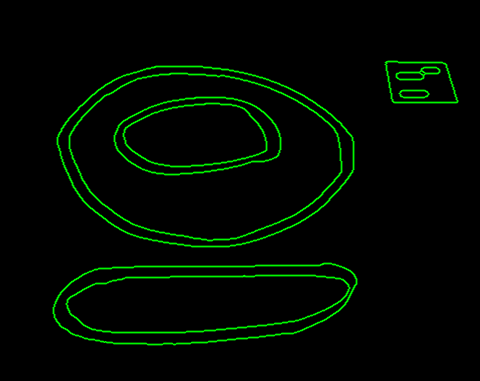
\includegraphics[scale=0.28]{pics/elimination/joinedAfterRemoval11.png}
		\caption{1 to 11}
		\label{construction11}
	\end{subfigure}
	\begin{subfigure}[t]{0.32\textwidth}
	\centering
		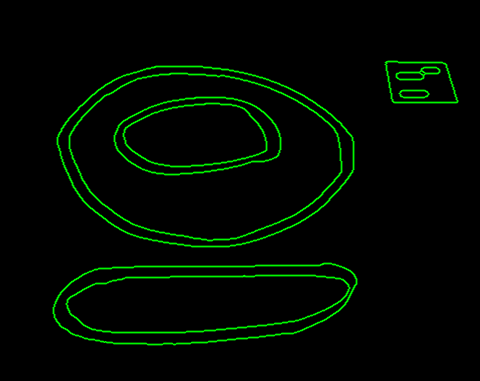
\includegraphics[scale=0.28]{pics/elimination/joinedAfterRemoval12.png}
		\caption{1 to 12}
		\label{construction12}
	\end{subfigure}
	\caption{Found Contours}
	\label{construction}
\end{figure}

............FINISH, SAY WHAT HAPPENS ON REMOVAL.
However, when by running several tests, on the sizes of contours discovered 
along with their sizes, it became apparent that all of the contours should be
kept. It was very possible that some of the smaller contours drawn by users 
would be even smaller than some of the contours detected by the algorithm. 
In this case setting a constant threshold for contour removal would not work
in the general case. By deciding to keep these contours, it also presented
other problems later on in the project. It may have been a better idea
delve down this path and have a dynamic assignment of a threshold based on
the average or lowest contour sizes. Using an average may not work if the user
intentionally draws one massive contour and several considerably smaller 
contours. The other option is to sort contour sizes and consider contours,
for example, were not needed if the sum of a subset of these contours, starting
from the largest, made up 90\% of the total contour size sum. This neglects 
contour hierarchy information, however, which is important to preserve, so
making a good algorithm for contour removal would require a lot more time
and investigation.\\
\\



...............FINISH, DO DOUBLE CONTOUR REMOVAL

\subsubsection{Determining Thresholds}
Throughout this project, there were numerous thresholds that I had to 
determine and set due to the importance of them in Computer Vision. 
As can be seen from the sections above, there was some degree of 
threshold testing that went into the decisions with threshold numbers.
The majority of the final constants were determined through observation
of test outputs. However, there are some ways in which the thresholding
could have been improved, the main areas I used thresholding are listed below.\\

\underline{\textbf{Canny Hysteresis Thresholds}}\\
\textbf{Test for determination:} Observation and binary search\\
\textbf{Problems:}\\ Limited to the set of landscape maps
				that the test was conducted on. In total
				there were 5 different maps tested drawn by 3 
				people, this was done without the ArUco marker
				present.\\
\textbf{Corrections/Alternatives:}\\
		Although the method has some solidity in its
		numbers, to make the thresholds even better, it
		would've been better if more landscape maps could
		have been tested, all including the ArUco marker. In
		addition, acquiring landscape maps from other user
		groups and having them drawn in different kinds of
		pen, over different coloured surfaces. Having 
		young children or industry specialists
		would be better as a wider range of drawings can be 
		analysed, possibly a better set of thresholds found. \\
\\
\underline{\textbf{Change detection Threshold}}\\
\textbf{Test for determination:} Trial and inspection\\
\textbf{Problems:}\\ I only went through this change detection with
				a black biro pen. As a result, the threshold I obtained
				from this was geared towards a thin pen. A 
				simple line drawn in marker pen, which is considerably thicker
				than biro, may cause enough change to prompt a rerender of
				the scene. Fitting the threshold for a thin pen means that
				to be counted as enough change, there has to be $X$ amount
				of pixels that have changed. Even a contour with large
				area will cause little change due to the amount of pixels
				the width of the biro pen will produce. The same amount
				can be attained by a smudge to a very thick marker pen which,
				to a human, is not enough to say there is a change in the
				scene.\\
\textbf{Corrections/Alternatives:}\\ A much better approach to this method
				would be to test for different utensils and attain a
				threshold in between. The better thing to do would be
				to have an adaptive thresholding depending on the environment,
				such as lighting, or drawing utensil chosen by the user.
				I go into more detail in the Section \ref{chapter:extensions}
				because this is a very important threshold for the project,
				especially if it a project of its kind is to be used 
				commercially. However, in retrospect, due to the fact the
				user will have to move their arm within the scene to draw
				any change onto the paper, this method will always work
				so long as the threshold is relatively low. Moving a whole
				arm into the scene will cause a large change in the 
				captured frames and so since this is a necessity (at the
				moment!) for change in the landscape map to happen, the
				level of precision for the change threshold, so long as
				it is lower than the amount of change an arm introduces,
				is sufficient. This may change in the future though, so
				is a point I thought I should mention in this evaluation. \\
\\
\underline{\textbf{Stabilisation}}\\
\textbf{Test for determination:} Counting Frames and in-situ observation\\
\textbf{Problems:}\\ There are two problems here, 
			one is that only a small set of people
			were tested and these from a certain age group.
			For example, a child might leave their arm in the picture a bit
			longer than most adults. In this scenario, it may be sufficient
			enough that the child is resting their arm in the scene for the
			prgoram to identify it as a stabilisation. This will cause 
			a rendering of something we do not want and is wasted computation.
			However, as soon as the child removes their arm and stabilisation
			met, there will be an accurate rendering. Thus, using this method
			the algorithm will always \textit{eventually} work. However,
			the amount of wasted computation may be an issue that can
			be avoided. The second problem is that the algorithm goes off
			a frame count basis. Since I only tested on two camera, it is
			unclear whether a bad camera with a bad framerate will cause
			a long wait between real world stabilisation and rerendering or
			a good camera with a fast framerate will wait too little time 
			after and consider a brief stall a stabilisationg due to the
			amount of frames it manages to capture.\\
\textbf{Corrections/Alternatives:}\\ The best way to solve these problems
			is to firstly, gather data on more users to determine their
			habits to set a time for stabilisation. To solve the second
			problem, testing on a few different cameras of different
			quality and adapting the algorithm to include
			an FPS measure to then use to set an
			adaptive threshold for stabilisation. This way, stabilisation
			be can proven more reliable on any hardware used. However,
			at this moment, since the algorithm eventually works and the
			two cameras I tested with were a standard laptop webcam and a
			mid/high end webcam, the frame count threshold shouldn't cause
			much issue with other hardware. This remains to be tested, however.\\
\\
\underline{\textbf{Explosion halting}}\\
\textbf{Test for determination:} Arbitrary assignment\\
\textbf{Problems:}\\ Explosion halting plays the important role 
				of describing when the program should render
				the landscape and when it should abandon it. This
				was arbitrarily set to 95\% of all points on the
				landscape being able to be assigned a height. However,
				whether this gives a good performance is completely
				random. For example, it may even have
				been sufficient to render with just 80\% of pixels
				being officially assigned a height. This means that
				a lot of the scenarios which the program currently 
				throws away may actually \textit{look} visually ok.
				This means, inherently, that the lower we can tolerate,
				the more resistant the program is to oddly detected 
				contour shapes. \\
\textbf{Corrections/Alternatives:}\\ A more controlled way to go about 
				setting this threshold should have been undergoing
				a lot of user testing at various levels of height 
				assignment success. My approach was simply to get a very
				accurate representation of heights so I set the threshold
				to a point of near perfect assignment. An alernative to
				this method is to allow a lower assignment but then
				convolve the result with some sort of neighbourhood 
				donation function which would assign estimates of the correct
				height to the pixels which weren't able to be reached
				through explosion. However, the speed of these methods
				would have to be measured against one another before any
				conclusions could be drawn.
				
				
\subsubsection{~TODO~ Height Map Creation}
Where most of the problems came up were upon height map creation. 
Creating the height map was the simplest way to 
describe the vertex heights when creating the 3D scene. The algorithm to
solve this problem involved being able to know where each pixel was in 
relation to the contours drawn by the user. The easiest way to do this is
find the contour that the pixel is within and assign the pixel a base
height equal to the level that the contour it is contained in is within
the hierarchy tree. Successfully able to create the tree and 
associate heights with contours, the problem to be solved was
identifying the contour any given pixel was within.\\
\\
After delving into the OpenCV documentation, I found a function
\texttt{pointPolygonTest} which would allow me to determine if a given
point was contained within a provided vector or points. 
I spent a long time calling this function 
but at a point realised that it does not working as expected.
When contours are detected, by \texttt{findContours()}, a hierarchy
is able to be returned, telling me how my contours were related in terms
of parents and containment. However, when using \texttt{pointPolygonTest()},
points that were obviously within a contour were not being identified
as being so. \\
\\
Looking into the problem, it seems that the errors begin higher up in the 
chain. OpenCV sometimes cannot tell whether a contour is closed, given a
set of the contour points. However, quite strangely, it is able to provide
a hierarchy of the points. Sometimes even when a contour is reported
as having children within the hierarchy, when a point is selected from within
that contour, calling \texttt{pointPolygonTest()} is not able to identify
the parent contour. This could be due to the way that the contours are
represented, as I stated before, they often backtrack and this backtracking
might cause an internal area which effecively lies on the contour line. Thus,
only points on the line will count as within a contour. The other theory
I had was on the behaviour of \texttt{pointPolygonTest()} which I found
online \footnote{http://code.opencv.org/issues/3648}, 
the ordering of the points within the supplied contours matters. After joining
contours together, this ordering is destroyed, not only that, but it also
ties into the backtracking issue. That even if I supplied one contour, the
fitted contour would be some sort of line, rather than a full ellipse
shape if it was identified as one contour (and closed) by OpenCV. The result
of this being that unless there is considerable manipulation of the contours
detected by OpenCV such that point order is preserved upon joining contours,
then supplying any contour that is not one originally found by OpenCV will
cause undefined behaviour for the \texttt{pointPolygonTest()} function.\\
\\
I tried two different approaches to try and solve the point containment issue,
these were both shape fitting algorithms offered by OpenCV. I first used
\texttt{fitEllipse()} to try and fit the minimum area, rotated ellipse to
the contours and would correct the errors post processing. However, after
implementing this method, although it was possible to tell which points belong
to which fitted rotated ellipse, the ellipse is stored as a minimum 
\textit{rectangle}, causing points that were not within the fitted contours
area to count as within that contour. In addition, ellipse fitting was less
than satisfactory and sometimes very large ellipses were fitted. In this case,
the corresponding bounding rectangles overlapped a lot in terms of area, making
containing contour assignment even more difficult. This approach was scrapped.\\
\\
The second approach was yo use the function \texttt{approxPolyDP()} which 
would fit a curve to a set of points and specify whether the area should be
closed. Fitting contours to found contour points seems very redundant but if
it would close the contours, it would be a satisfactory method. Implementing
this solution did close the contours but in a way that was incorrect. 
Due to the fact that I joined contours together without any restructure
of internal points, the order of points was preserved. Since it is the case
that \texttt{approcPolyDP()} takes into account the order of points passed
to it, the following result was obtained ...

..........APPrOXIMATE CONTOURS FROM POINTs


Due to the time constraints on the project, I had decided to leave this issue
behind me and approach it in my own way. At the time I evaluated that spending
more time to investigate the problem and maybe or maybe not find a solution
that could even require changing more logic around my contour joining was
not the best choice I could have made. I stand by the decision, though if
I had more time, investigating down this route is definitely something I should
have done. There were a number of different methods I tried before
settling.\\
\\
The approach I took was to perform a linear traversal through
the image with known contour pixels. Based on whether I encountered a 
contour pixel on traversal, I could tell which contour I was in, very simply
from the property that all contours should be closed. Take any strip 
of pixels (as they are the smallest unit of display), I maintain a stack which
tells me which contour I am currently within. I pop from the stack when I
meet the contour once again. This accurately tells me the contour level I am
within without needing $n^2$ calls to the \texttt{pointPolygonTest()} function
which does not give me my required answer almost all the time.\\
\\
Further delving into this algorithm, another problem occurred where
if our strip of pixels is on a tangent to the contour edge, the stack method
does not work. This causes inconsistencies in the height assignment. Luckily,
this happens only after we encounter the first tangent point. To correct this,
the strip is noted down in a list, after traversal, a blurring kernel is
convolved with these lists to correctly identify which contour each point
in the image was situated within.\\
\\
The next problem in this string of issues was to interpolate the heights
each pixel should have. The heights should get closer toward the next 
contour level height as that contour is approached. Again, 
\texttt{pointPolygonTest()} offers this functionality but it does not work
accurately, nor does it always return correct answers due to its defined
behaviour. To solve this I approached the problem with a breadth first 
search algorithm called "explosion"
that converges to the correct answer, however, the algorithm
requires several passes over the entire image, especially if the 
contours have a large area. The 
current run time of the algorithm is heavily dependent on the area
of the contours that the user draws. A larger area will incur a larger
run time for this algorithm which is not ideal. 
An alternative to this method was
to use euclidean distance transforms, offered also by OpenCV. The breadth
first search algorithm works on a very similar basis except distances
are more discretised as "distance in pixels" is a whole number. However,
I was very skeptical of its accuracy after the original issues with
\texttt{pointPolygonTest()} so went onto implement my solution which does produce
the correct answer. In addition, there were various issues with the function
that I have highlighted in \ref{chapter:implementation}. 
However, after implenting my algorithm and testing its run time,
the computation does take a while and it is
to my regret I did not have the time to go back and try this method and
compare run times between the two algorithms.


\end{document}